\def\topic{Classes and Objects - 2}
\input{comp125lectureHeader}

\section{Overview}

    We explore classes and objects in more detail on the following points:
    
    \begin{itemize}
    \item \texttt{this} keyword
    \item Comparing objects
    \item Unit testing methods of a class
    \item \texttt{static} vs instance members
    \item Manipulating references
    \end{itemize}
 
 
\section{\texttt{this} keyword}
  Consider the following class definition,
 
\begin{lstlisting}[frame=single,style=buggy]
public class Circle {
  private double @radius@;
  public void setRadius(double @radius@) {
    @radius@ = @Math.abs(radius)@;
  }
  //assume getter is also defined
}
\end{lstlisting}  

Because the parameter and instance variable have the same name (\texttt{radius}), it is not clear which one is affected in the assignment statement on line 4 above.
\vskip 0.5cm
Java provides a keyword \texttt{this} that refers to the calling object and gives access to its instance variables and methods. 
  \begin{lstlisting}[frame=single,style=correct]
public class Circle {
  private double @radius@;
  public void setRadius(double radius) {
    @this@.radius = Math.abs(radius);
  }
  //assume getter is also defined
}
  \end{lstlisting}  
  Line 4 now shows that the instance variable \texttt{radius} on line 2 will be affected by the assignment statement. As you can see, the \texttt{Math.abs} method  is using the parameter variable \texttt{radius}.

\begin{exercise}[6][Disambiguate assignment operation]
Get rid of the ambiguity in the \texttt{setSide} method
\begin{lstlisting}[frame=single,style=buggy]
public class Square {
  private double side;
  public void setSide(double side) {
    side = Math.max(0, side);
  }
  //assume getter is also defined
}
\end{lstlisting}  	
\end{exercise}
\begin{answer} 
\begin{lstlisting}
public class Square {
  private double side;
  public void setSide(double side) {
    @this.side@ = Math.max(0, side);
  }
  //assume getter is also defined
}
\end{lstlisting} 
\end{answer}


\section{Comparing objects (\texttt{compareTo} method)}

The method \texttt{compareTo} provides a way to define an order on two objects (say $a$ and $b$). The method is called on object $a$ and the object $b$ is passed as a parameter, the result indicating how $a$ compares to $b$.

\begin{flag}
You can access \texttt{private} instance members of the object passed inside a method directly, as long as the object is of the same class as the one the method is in.	
\end{flag}


  Consider the following method in the \texttt{Circle} class,
  \begin{lstlisting}[style=correct,basicstyle=\footnotesize]
  public class Circle {
    // other methods and instance members
    
    /* 
    comparison criterion: radius.
    return 1 if the calling object is ``more'' than other 
    -1 if its ``less''
     0 if they are ``equal'' 
     */
    public int compareTo(Circle other) {
        if(this.radius > other.radius)
  	      return 1;
        if(this.radius < other.radius)
          return -1;
        return 0; 
    }
  }
  \end{lstlisting}    
\clearpage
\subsection{\texttt{compareTo} in action}
  \begin{lstlisting}[frame=single,style=correct,basicstyle=\footnotesize]
  Circle myCircle = new Circle(12);
  Circle yourCircle = new Circle(18);
  Circle ourCircle = new Circle(7);
  Circle theirCircle = new Circle(12);
  
  int s1 = myCircle.compareTo(yourCircle); //-1
  int s2 = myCircle.compareTo(ourCircle); //1
  int s3 = myCircle.compareTo(theirCircle); //0
  int s4 = theirCircle.compareTo(ourCircle); // ??
  int s5 = ourCircle.compareTo(yourCircle); // ??
  int s6 = yourCircle.compareTo(yourCircle); // ??
  \end{lstlisting}  

\begin{exercise}[6][Implement \texttt{compareTo} method]
Add a \texttt{compareTo} method in class Square that returns,

\begin{itemize}
\item 1 if calling object's area is more than parameter object's area 
\item -1 if calling object's area is less than parameter object's area 
\item 0 if calling object's area is equal to parameter object's area 
\end{itemize}
\begin{lstlisting}[frame=single,style=buggy]
public class Square {
  private double side;
  //assume getter and setter
  public double area() {
    return side * side;
  }
}
\end{lstlisting}  	
\end{exercise}
\begin{answer} \begin{lstlisting}
public int compareTo(Square other) {
	if(area() > other.area())
		return 1;
	if(area() < other.area())
		return -1;
	//in all other cases:
	return 0;
}
\end{lstlisting} \end{answer}  
  
%\section{The \texttt{equals} method}
%  If we define \texttt{compareTo}, then \texttt{equals} becomes very simple (provided comparison criteria are the same).
%  \begin{lstlisting}[frame=single,style=correct]
%public class Circle {
%  //other parts (including compareTo)
%  public boolean equals(Circle other) {
%    return compareTo(other) == 0;
%  }
%}
%\end{lstlisting}    
%
%\clearpage
%\subsection{\texttt{equals} in action}
%  \begin{lstlisting}[frame=single,style=correct,basicstyle=\footnotesize]
%  Circle myCircle = new Circle(12);
%  Circle yourCircle = new Circle(18);
%  Circle ourCircle = new Circle(7);
%  Circle theirCircle = new Circle(12);
%  
%  boolean t1 = myCircle.equals(yourCircle); //false
%  boolean t2 = myCircle.equals(ourCircle); //false
%  boolean t3 = myCircle.equals(theirCircle); //true
%  boolean t4 = theirCircle.equals(ourCircle); //??
%  boolean t5 = ourCircle.equals(yourCircle); //??
%  boolean t6 = yourCircle.equals(yourCircle); //??
%  \end{lstlisting}  
%  
%\begin{exercise}[6][Implement \texttt{equals} method]
%Add a \texttt{equals} method in class Square that returns:
%
%\begin{itemize}
%\item \texttt{true} if calling object and parameter object have the same values of instance variable \texttt{side}
%\item \texttt{false} otherwise
%\end{itemize}
%
%Assume compareTo has not been defined.
%\begin{lstlisting}[frame=single,style=buggy]
%public class Square {
%  private double side;
%  //assume getter and setter
%}
%\end{lstlisting}  	
%\end{exercise}  
%\begin{answer} \begin{lstlisting}
%public boolean equals(Square other) {
%	if(side == other.side)
%		return true;
%	else
%		return false;
%}
%\end{lstlisting} \end{answer}

\section{Multi-criteria comparison}
  What happens if there are multiple levels of comparison criteria? For example, if we compare two rectangles based on area, but they have the same area, we then compare them on perimeter, and if even that's the same, return 0. 

\begin{exercise}[7][Implement multi-criteria\texttt{compareTo} method]
Add a \texttt{compareTo} method in class \texttt{Rectangle} that returns,

\begin{itemize}
\item 1 if calling object's area is more than parameter object's area, or if they have the same area, but calling object's perimeter is more than parameter object's perimeter.
\item -1 if calling object's area is less than parameter object's area, or if they have the same area, but calling object's perimeter is less than parameter object's perimeter.
\item 0 if calling object's area is equal to parameter object's area and calling object's perimeter is equal to parameter object's perimeter. 
\end{itemize}
\begin{lstlisting}[frame=single,style=buggy]
public class Rectangle {
  private double width, height;
  //assume getters and setters
  public double area() { return width * height; }
  public double perimeter() { return 2*(width + height); }
}
\end{lstlisting}  	
\end{exercise}
\begin{answer} \begin{lstlisting}
public int compareTo(Rectangle other) {
	//first key comparison
	if(area() > other.area())
		return 1;
	if(area() < other.area())
		return -1;
	
	//second key comparison
	if(perimeter() > other.perimeter())
		return 1;
	if(perimeter() < other.perimeter())
		return -1;
	
	//still nothing?
	return 0;
}
\end{lstlisting} \end{answer}

\section{Unit testing methods of a class}

An example class with a method that will not produce the expected result in all situations.
  \begin{lstlisting}[frame=single,style=buggy]
public class Line {
  private int x1, y1, x2, y2;
  //other parts
  public double getMidX() {
    return x1+x2/2; //i know.
  }
}
  \end{lstlisting}    


\section{JUnit testing}
  JUnit provides a framework for testing individual methods. It works based on following assertions:
  
\begin{enumerate}
  \item \texttt{assertEquals(expected double, double returned by method, tolerance)}: 

passes if,

\begin{verbatim}
Math.abs(expected double - double returned by method) <= tolerance
\end{verbatim}

  \item \texttt{assertEquals(expected integer, integer returned by method)}: passes if,

\begin{verbatim}
expected integer == integer returned by method
\end{verbatim}

  \item \texttt{assertTrue(boolean value)}: passes if parameter is \texttt{true}.
  \item \texttt{assertTrue(boolean value)}: passes if parameter is \texttt{false}.
  \item \texttt{assertNull(Object/array)}: passes if parameter is \texttt{null}.
  \item \texttt{assertNotNull(Object/array)}: passes if parameter is \textbf{NOT} \texttt{null}.
  \item More assertions can be found at: 

\href{http://junit.org/junit4/javadoc/latest/org/junit/Assert.html}{http://junit.org/junit4/javadoc/latest/org/junit/Assert.html}

\end{enumerate}
  
\begin{lstlisting}[style=junit]

import static org.junit.Assert.*;
import org.junit.Test;
public class LineTest {
  @Test
  public void testGetMidX() {
    Line a = new Line(0, 10, 8, 12);
    assertEquals(4, a.getMidX(), 0.001); //passes
    Line b = new Line(5, 10, 6, 12);
    assertEquals(5.5, b.getMidX(), 0.001); //fails
}
\end{lstlisting}    

\newpage

\subsubsection{Corrected version by looking at JUnit failure}
  \begin{lstlisting}[frame=single,style=correct]
public class Line {
  private int x1, y1, x2, y2;
  //other parts
  public double getMidX() {
    return @(x1+x2)/2.0@; 
  }
}
  \end{lstlisting}   

\section{Static members vs. Instance members}
Static members are the ones that are accessed in the context of a class. You don't need to create objects of that class in order to access them. For example, consider the number of eyes \textbf{dinosaurs} have. Note, we didn't say, how many eyes does Dorothy the dinosaur, or Tyrone the dinosaur have. 
\vskip 0.5cm
We don't even need any dinosaur to be alive to answer that question, since it's an attribute of the \emph{collective} (the class) rather than an \emph{individual} (an object).
\vskip 0.5cm
On the other hand, the variables \texttt{weight, height} are different for each dinosaur that was there. Hence, they are \emph{instance variables}. Similarly, the body mass index (defined as weight divided by square of height) is an \emph{instance method}, that must be called on an \emph{individual} (the object), not the \emph{collective} (the class)
\vskip 0.5cm
Consider the following class:

\begin{lstlisting}[style=buggy,basicstyle=\footnotesize]
class Dinosaur {
  public @static@ int nEyes = 2;
  public @static@ int nEars = 2;
  public @static@ double eyesToEarsRatio() {
	return nEyes * 1.0 / nEars;
  }
  
  private double weight, height;
  //assume getters, setters
  //assume parameterized constructors
  public double bodyMassIndex() {
    return weight/(height*height);
  }
}
\end{lstlisting}

\subsection{Static member access}

\begin{lstlisting}[style=buggy]
int eyeCount = @Dinosaur@.nEyes;
double prop = @Dinosaur@.eyesToEarsRatio();
\end{lstlisting} 

\newpage
\subsection{Instance member access}

\begin{lstlisting}[style=buggy]
Dinosaur dorothy = new Dinosaur(450,3.6);
double w = @dorothy@.getWeight();
double h = @dorothy@.getHeight();
double bmi = @dorothy@.bodyMassIndex();
\end{lstlisting}

Note that in this example the instance variables are private, otherwise (if they were public), they could be accessed in the same way (on a calling object).

\begin{exercise}[5][Accessing static and instance members]
Display the members \texttt{data1, data2, method1, method2} of class \texttt{MyClass} (or object \texttt{obj} of class \texttt{MyClass}) in the client code.

\begin{lstlisting}[frame=single,style=buggy]
public class MyClass {
	public int data1;
	public static int data2;
	public static int method1() { return data2; }
	public int method2() { return data1; }
}

class Client {
	public static void main(String[] args) {
		MyClass obj = new MyClass();
		//your code	
	}
}
\end{lstlisting}  	
\end{exercise}
\begin{answer} \begin{lstlisting}
//instance variable called on object
System.out.println(obj.data1); 

//static variable called on class
System.out.println(MyClass.data2); 

//static method called on class
System.out.println(MyClass.method1()); 

//instance method called on object 
System.out.println(obj.method2()); 
\end{lstlisting} \end{answer}

\subsection{Typical static methods}
Typically, methods are classified as static, if the values they operate on are passed to the methods. For example:

\begin{lstlisting}[basicstyle=\footnotesize]
class StringService {
  public static char lastItem(String s) {
    if(s == null || s.length() == 0)
      return (char)0;
    return s.charAt(s.length() - 1);
  }
 }
\end{lstlisting}

\begin{lstlisting}[basicstyle=\footnotesize]
class IntegerService {
	public static int getNumberOfDigits(int num) {
		if(num == 0)
			return 0;
		// Remove any sign from number, 
		// add it to an empty string, 
		// return its length.
		return (Math.abs(num) + "").length();
	}
}
\end{lstlisting}

\section{Manipulating references}

\subsection{Shallow copy}
  Consider the following class definition and client code:
  
  \begin{lstlisting}
  public class Circle {
  	private double radius;
  	//other parts
  }
  \end{lstlisting}    
  
  \begin{lstlisting}[style=correct,basicstyle=\footnotesize]
  Circle c = new Circle(30);
  Circle d = c; 
  //c and d refer to same
  //instance variable space
  d.setRadius(50);
  System.out.println(c.getRadius()); //??
  \end{lstlisting}    

  Object \texttt{d} holds reference to the same physical object as \texttt{c}. Therefore, when the \texttt{radius} of object \texttt{d} is modified, \texttt{radius} of object \texttt{c} also gets updated.

%  \begin{center}
%%  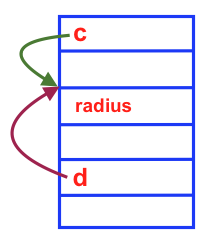
\includegraphics[scale=0.5]{images/shallowCopy.png}
%	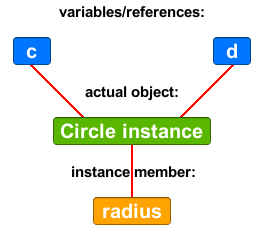
\includegraphics[scale=1]{images/shallowObjRef.png}
%  \end{center}

\begin{center}
<img src="./../fig/classesObjects/classesObjects-ClassUMLDiagram.png" alt="Drawing" width = "400"/>
\end{center}

Let's say, \texttt{c} changes to \texttt{null}.

\begin{center}
<img src="./../fig/classesObjects/classesObjects-ClassUMLDiagram.png" alt="Drawing" width = "400"/>
\end{center}
  
\begin{exercise}[5][Create a shallow copy]
Create a shallow copy of \texttt{myObj} into \texttt{yourObj}. Increase the radius of \texttt{yourObj} by 2. What is the new radius of \texttt{myObj}?

\begin{lstlisting}[frame=single,style=buggy,backgroundcolor = \color{green!10!white}]
public class Circle {
	private double radius;
	//assume getters, setters 
	// and constructors defined
}

class Client {
	public static void main(String[] args) {
		Circle myObj = new Circle(1.5);
		//your code
	}
}
\end{lstlisting}  	
\end{exercise}
\begin{answer} \begin{lstlisting}
Circle yourObj = myObj; //shallow copy
youObj.setRadius(yourObj.getRadius() + 2);
System.out.println(myObj.getRadius()); //will be 3.5
\end{lstlisting} \end{answer}


\subsection{Deep copy}
  \begin{lstlisting}[style=correct,basicstyle=\footnotesize]
  Circle c = new Circle(30);
  Circle d = new Circle();
  d.setRadius(c.getRadius());
  //c's radius copied into d's radius
  System.out.println(c.getRadius()); //??
  \end{lstlisting}    
  
  Object \texttt{d} is a clone of object \texttt{c}. Object \texttt{c} and \texttt{d} are independent objects. Modifying one does not alter the other.

\begin{center}
<img src="./../fig/classesObjects/classesObjects-ClassUMLDiagram.png" alt="Drawing" width = "400"/>
\end{center}

%  \begin{center}
%  %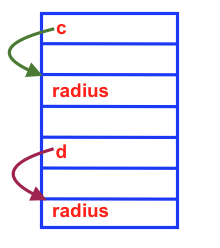
\includegraphics[scale=0.5]{images/deepCopy}
%  	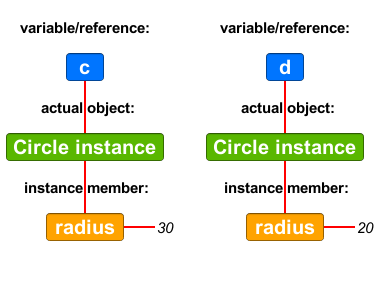
\includegraphics[scale=1]{images/deepObjCopy.png}
%  \end{center}
  
\begin{exercise}[3][Create a deep copy]
Create a deep copy of \texttt{myObj} into \texttt{yourObj}. Increase the radius of \texttt{yourObj} by 2. What is the new radius of \texttt{myObj}?

\begin{lstlisting}[frame=single,style=buggy]
public class Circle {
	private double radius;
	//assume getters, setters
	// and constructors defined
}

class Client {
	public static void main(String[] args) {
		Circle myObj = new Circle(1.5);
		//your code
	}
}
\end{lstlisting}  	
\end{exercise}

\begin{answer} \begin{lstlisting}
//create a brand-spanking new object in memory
Circle yourObj = new Circle(); 
//get the value for radius from myObj
yourObj.setRadius(myObj.getRadius());
youObj.setRadius(yourObj.getRadius() + 2);
System.out.println(myObj.getRadius()); //will still be 1.5
\end{lstlisting} \end{answer}

\clearpage
\subsection{Copy constructor}
  \begin{lstlisting}
  public class Circle {
  	private double radius;
  	//setters, getters
 
  	public Circle(double radius) {
		setRadius(radius);
  	}
	
	public Circle(Circle other) {
		setRadius(other.radius);
  	}
  }
  \end{lstlisting}   
  
\begin{exercise}[5][Define a copy constructor]
Define a copy constructor in class \texttt{Rectangle}. 

\begin{lstlisting}[frame=single,style=buggy]
public class Rectangle {
	private double width, height;
	//assume getters, setters defined
	//define copy constructor here
}
\end{lstlisting}  	
\end{exercise} 
\begin{answer} \begin{lstlisting}
public Rectangle(Rectangle source) {
	setWidth(source.getWidth());
	setHeight(source.getHeight());
}
\end{lstlisting} \end{answer}

\subsubsection{Copy constructor call} 
  \begin{lstlisting}
  Circle c = new Circle(30);
  Circle d = new Circle(c);
  \end{lstlisting} 

\begin{exercise}[5][Call a copy constructor]
Deep copy \texttt{myObj} into \texttt{yourObj} using the copy constructor defined in class \texttt{Square}. 

\begin{lstlisting}[frame=single,style=buggy]
public class Square {
	private double side;
	//assume getters, setters defined
	public Square(Square other) {
		setSide(other.side);
	}
}

class Client {
	public static void main(String[] args) {
		Square myObj = new Square(2.4);
		//your code
	}
}
\end{lstlisting}  	
\end{exercise}
\begin{answer} \begin{lstlisting}
Square yourObj = new Square(myObj);
\end{lstlisting} \end{answer}

\input{comp125lectureFooter}exer
